
%% bare_conf.tex
%% V1.3
%% 2007/01/11
%% by Michael Shell
%% See:
%% http://www.michaelshell.org/
%% for current contact information.
%%
%% This is a skeleton file demonstrating the use of IEEEtran.cls
%% (requires IEEEtran.cls version 1.7 or later) with an IEEE conference paper.
%%
%% Support sites:
%% http://www.michaelshell.org/tex/ieeetran/
%% http://www.ctan.org/tex-archive/macros/latex/contrib/IEEEtran/
%% and
%% http://www.ieee.org/

%%*************************************************************************
%% Legal Notice:
%% This code is offered as-is without any warranty either expressed or
%% implied; without even the implied warranty of MERCHANTABILITY or
%% FITNESS FOR A PARTICULAR PURPOSE! 
%% User assumes all risk.
%% In no event shall IEEE or any contributor to this code be liable for
%% any damages or losses, including, but not limited to, incidental,
%% consequential, or any other damages, resulting from the use or misuse
%% of any information contained here.
%%
%% All comments are the opinions of their respective authors and are not
%% necessarily endorsed by the IEEE.
%%
%% This work is distributed under the LaTeX Project Public License (LPPL)
%% ( http://www.latex-project.org/ ) version 1.3, and may be freely used,
%% distributed and modified. A copy of the LPPL, version 1.3, is included
%% in the base LaTeX documentation of all distributions of LaTeX released
%% 2003/12/01 or later.
%% Retain all contribution notices and credits.
%% ** Modified files should be clearly indicated as such, including  **
%% ** renaming them and changing author support contact information. **
%%
%% File list of work: IEEEtran.cls, IEEEtran_HOWTO.pdf, bare_adv.tex,
%%                    bare_conf.tex, bare_jrnl.tex, bare_jrnl_compsoc.tex
%%*************************************************************************

% *** Authors should verify (and, if needed, correct) their LaTeX system  ***
% *** with the testflow diagnostic prior to trusting their LaTeX platform ***
% *** with production work. IEEE's font choices can trigger bugs that do  ***
% *** not appear when using other class files.                            ***
% The testflow support page is at:
% http://www.michaelshell.org/tex/testflow/



% Note that the a4paper option is mainly intended so that authors in
% countries using A4 can easily print to A4 and see how their papers will
% look in print - the typesetting of the document will not typically be
% affected with changes in paper size (but the bottom and side margins will).
% Use the testflow package mentioned above to verify correct handling of
% both paper sizes by the user's LaTeX system.
%
% Also note that the "draftcls" or "draftclsnofoot", not "draft", option
% should be used if it is desired that the figures are to be displayed in
% draft mode.
%
\documentclass[conference]{IEEEtran}
% Add the compsoc option for Computer Society conferences.
%
% If IEEEtran.cls has not been installed into the LaTeX system files,
% manually specify the path to it like:
% \documentclass[conference]{../sty/IEEEtran}





% Some very useful LaTeX packages include:
% (uncomment the ones you want to load)


% *** MISC UTILITY PACKAGES ***
%
%\usepackage{ifpdf}
% Heiko Oberdiek's ifpdf.sty is very useful if you need conditional
% compilation based on whether the output is pdf or dvi.
% usage:
% \ifpdf
%   % pdf code
% \else
%   % dvi code
% \fi
% The latest version of ifpdf.sty can be obtained from:
% http://www.ctan.org/tex-archive/macros/latex/contrib/oberdiek/
% Also, note that IEEEtran.cls V1.7 and later provides a builtin
% \ifCLASSINFOpdf conditional that works the same way.
% When switching from latex to pdflatex and vice-versa, the compiler may
% have to be run twice to clear warning/error messages.






% *** CITATION PACKAGES ***
%
%\usepackage{cite}
% cite.sty was written by Donald Arseneau
% V1.6 and later of IEEEtran pre-defines the format of the cite.sty package
% \cite{} output to follow that of IEEE. Loading the cite package will
% result in citation numbers being automatically sorted and properly
% "compressed/ranged". e.g., [1], [9], [2], [7], [5], [6] without using
% cite.sty will become [1], [2], [5]--[7], [9] using cite.sty. cite.sty's
% \cite will automatically add leading space, if needed. Use cite.sty's
% noadjust option (cite.sty V3.8 and later) if you want to turn this off.
% cite.sty is already installed on most LaTeX systems. Be sure and use
% version 4.0 (2003-05-27) and later if using hyperref.sty. cite.sty does
% not currently provide for hyperlinked citations.
% The latest version can be obtained at:
% http://www.ctan.org/tex-archive/macros/latex/contrib/cite/
% The documentation is contained in the cite.sty file itself.






% *** GRAPHICS RELATED PACKAGES ***
%
\ifCLASSINFOpdf
  % \usepackage[pdftex]{graphicx}
  % declare the path(s) where your graphic files are
  % \graphicspath{{../pdf/}{../jpeg/}}
  % and their extensions so you won't have to specify these with
  % every instance of \includegraphics
  % \DeclareGraphicsExtensions{.pdf,.jpeg,.png}
\else
  % or other class option (dvipsone, dvipdf, if not using dvips). graphicx
  % will default to the driver specified in the system graphics.cfg if no
  % driver is specified.
  % \usepackage[dvips]{graphicx}
  % declare the path(s) where your graphic files are
  % \graphicspath{{../eps/}}
  % and their extensions so you won't have to specify these with
  % every instance of \includegraphics
  % \DeclareGraphicsExtensions{.eps}
\fi
% graphicx was written by David Carlisle and Sebastian Rahtz. It is
% required if you want graphics, photos, etc. graphicx.sty is already
% installed on most LaTeX systems. The latest version and documentation can
% be obtained at: 
% http://www.ctan.org/tex-archive/macros/latex/required/graphics/
% Another good source of documentation is "Using Imported Graphics in
% LaTeX2e" by Keith Reckdahl which can be found as epslatex.ps or
% epslatex.pdf at: http://www.ctan.org/tex-archive/info/
%
% latex, and pdflatex in dvi mode, support graphics in encapsulated
% postscript (.eps) format. pdflatex in pdf mode supports graphics
% in .pdf, .jpeg, .png and .mps (metapost) formats. Users should ensure
% that all non-photo figures use a vector format (.eps, .pdf, .mps) and
% not a bitmapped formats (.jpeg, .png). IEEE frowns on bitmapped formats
% which can result in "jaggedy"/blurry rendering of lines and letters as
% well as large increases in file sizes.
%
% You can find documentation about the pdfTeX application at:
% http://www.tug.org/applications/pdftex





% *** MATH PACKAGES ***
%
%\usepackage[cmex10]{amsmath}
% A popular package from the American Mathematical Society that provides
% many useful and powerful commands for dealing with mathematics. If using
% it, be sure to load this package with the cmex10 option to ensure that
% only type 1 fonts will utilized at all point sizes. Without this option,
% it is possible that some math symbols, particularly those within
% footnotes, will be rendered in bitmap form which will result in a
% document that can not be IEEE Xplore compliant!
%
% Also, note that the amsmath package sets \interdisplaylinepenalty to 10000
% thus preventing page breaks from occurring within multiline equations. Use:
%\interdisplaylinepenalty=2500
% after loading amsmath to restore such page breaks as IEEEtran.cls normally
% does. amsmath.sty is already installed on most LaTeX systems. The latest
% version and documentation can be obtained at:
% http://www.ctan.org/tex-archive/macros/latex/required/amslatex/math/





% *** SPECIALIZED LIST PACKAGES ***
%
%\usepackage{algorithmic}
% algorithmic.sty was written by Peter Williams and Rogerio Brito.
% This package provides an algorithmic environment fo describing algorithms.
% You can use the algorithmic environment in-text or within a figure
% environment to provide for a floating algorithm. Do NOT use the algorithm
% floating environment provided by algorithm.sty (by the same authors) or
% algorithm2e.sty (by Christophe Fiorio) as IEEE does not use dedicated
% algorithm float types and packages that provide these will not provide
% correct IEEE style captions. The latest version and documentation of
% algorithmic.sty can be obtained at:
% http://www.ctan.org/tex-archive/macros/latex/contrib/algorithms/
% There is also a support site at:
% http://algorithms.berlios.de/index.html
% Also of interest may be the (relatively newer and more customizable)
% algorithmicx.sty package by Szasz Janos:
% http://www.ctan.org/tex-archive/macros/latex/contrib/algorithmicx/




% *** ALIGNMENT PACKAGES ***
%
%\usepackage{array}
% Frank Mittelbach's and David Carlisle's array.sty patches and improves
% the standard LaTeX2e array and tabular environments to provide better
% appearance and additional user controls. As the default LaTeX2e table
% generation code is lacking to the point of almost being broken with
% respect to the quality of the end results, all users are strongly
% advised to use an enhanced (at the very least that provided by array.sty)
% set of table tools. array.sty is already installed on most systems. The
% latest version and documentation can be obtained at:
% http://www.ctan.org/tex-archive/macros/latex/required/tools/


%\usepackage{mdwmath}
%\usepackage{mdwtab}
% Also highly recommended is Mark Wooding's extremely powerful MDW tools,
% especially mdwmath.sty and mdwtab.sty which are used to format equations
% and tables, respectively. The MDWtools set is already installed on most
% LaTeX systems. The lastest version and documentation is available at:
% http://www.ctan.org/tex-archive/macros/latex/contrib/mdwtools/


% IEEEtran contains the IEEEeqnarray family of commands that can be used to
% generate multiline equations as well as matrices, tables, etc., of high
% quality.


%\usepackage{eqparbox}
% Also of notable interest is Scott Pakin's eqparbox package for creating
% (automatically sized) equal width boxes - aka "natural width parboxes".
% Available at:
% http://www.ctan.org/tex-archive/macros/latex/contrib/eqparbox/





% *** SUBFIGURE PACKAGES ***
%\usepackage[tight,footnotesize]{subfigure}
% subfigure.sty was written by Steven Douglas Cochran. This package makes it
% easy to put subfigures in your figures. e.g., "Figure 1a and 1b". For IEEE
% work, it is a good idea to load it with the tight package option to reduce
% the amount of white space around the subfigures. subfigure.sty is already
% installed on most LaTeX systems. The latest version and documentation can
% be obtained at:
% http://www.ctan.org/tex-archive/obsolete/macros/latex/contrib/subfigure/
% subfigure.sty has been superceeded by subfig.sty.



%\usepackage[caption=false]{caption}
%\usepackage[font=footnotesize]{subfig}
% subfig.sty, also written by Steven Douglas Cochran, is the modern
% replacement for subfigure.sty. However, subfig.sty requires and
% automatically loads Axel Sommerfeldt's caption.sty which will override
% IEEEtran.cls handling of captions and this will result in nonIEEE style
% figure/table captions. To prevent this problem, be sure and preload
% caption.sty with its "caption=false" package option. This is will preserve
% IEEEtran.cls handing of captions. Version 1.3 (2005/06/28) and later 
% (recommended due to many improvements over 1.2) of subfig.sty supports
% the caption=false option directly:
%\usepackage[caption=false,font=footnotesize]{subfig}
%
% The latest version and documentation can be obtained at:
% http://www.ctan.org/tex-archive/macros/latex/contrib/subfig/
% The latest version and documentation of caption.sty can be obtained at:
% http://www.ctan.org/tex-archive/macros/latex/contrib/caption/




% *** FLOAT PACKAGES ***
%
%\usepackage{fixltx2e}
% fixltx2e, the successor to the earlier fix2col.sty, was written by
% Frank Mittelbach and David Carlisle. This package corrects a few problems
% in the LaTeX2e kernel, the most notable of which is that in current
% LaTeX2e releases, the ordering of single and double column floats is not
% guaranteed to be preserved. Thus, an unpatched LaTeX2e can allow a
% single column figure to be placed prior to an earlier double column
% figure. The latest version and documentation can be found at:
% http://www.ctan.org/tex-archive/macros/latex/base/



%\usepackage{stfloats}
% stfloats.sty was written by Sigitas Tolusis. This package gives LaTeX2e
% the ability to do double column floats at the bottom of the page as well
% as the top. (e.g., "\begin{figure*}[!b]" is not normally possible in
% LaTeX2e). It also provides a command:
%\fnbelowfloat
% to enable the placement of footnotes below bottom floats (the standard
% LaTeX2e kernel puts them above bottom floats). This is an invasive package
% which rewrites many portions of the LaTeX2e float routines. It may not work
% with other packages that modify the LaTeX2e float routines. The latest
% version and documentation can be obtained at:
% http://www.ctan.org/tex-archive/macros/latex/contrib/sttools/
% Documentation is contained in the stfloats.sty comments as well as in the
% presfull.pdf file. Do not use the stfloats baselinefloat ability as IEEE
% does not allow \baselineskip to stretch. Authors submitting work to the
% IEEE should note that IEEE rarely uses double column equations and
% that authors should try to avoid such use. Do not be tempted to use the
% cuted.sty or midfloat.sty packages (also by Sigitas Tolusis) as IEEE does
% not format its papers in such ways.





% *** PDF, URL AND HYPERLINK PACKAGES ***
%
%\usepackage{url}
% url.sty was written by Donald Arseneau. It provides better support for
% handling and breaking URLs. url.sty is already installed on most LaTeX
% systems. The latest version can be obtained at:
% http://www.ctan.org/tex-archive/macros/latex/contrib/misc/
% Read the url.sty source comments for usage information. Basically,
% \url{my_url_here}.





% *** Do not adjust lengths that control margins, column widths, etc. ***
% *** Do not use packages that alter fonts (such as pslatex).         ***
% There should be no need to do such things with IEEEtran.cls V1.6 and later.
% (Unless specifically asked to do so by the journal or conference you plan
% to submit to, of course. )

\usepackage[pdftex]{graphicx}

\usepackage{amsmath}
\usepackage{amssymb}

\usepackage{multirow}
\usepackage{listings}
\usepackage{booktabs}
\usepackage{tikz}
\usepackage{xspace}

\newtheorem{theorem}{Theorem}
\newtheorem{definition}{Definition}

% correct bad hyphenation here
\hyphenation{op-tical net-works semi-conduc-tor}

\newcommand{\whoop}{\textsc{Whoop}\xspace}
\newcommand{\corral}{\textsc{Corral}\xspace}

\newcommand{\ADComment}[1]{\textcolor{blue}{Ally: #1}}
\newcommand{\PDComment}[1]{\textcolor{magenta}{Pantazis: #1}}

\begin{document}
%
% paper title
% can use linebreaks \\ within to get better formatting as desired
\title{Static Lockset Analysis for Accelerating\\ Bug Finding in Linux Kernel Modules}


% author names and affiliations
% use a multiple column layout for up to three different
% affiliations
\author{\IEEEauthorblockN{Pantazis Deligiannis}
\IEEEauthorblockA{Department of Computing,\\
Imperial College London, UK\\
p.deligiannis@imperial.ac.uk}
\and
\IEEEauthorblockN{Alastair F. Donaldson}
\IEEEauthorblockA{Department of Computing,\\
Imperial College London, UK\\
alastair.donaldson@imperial.ac.uk}
\and
\IEEEauthorblockN{Zvonimir Rakamari\'c}
\IEEEauthorblockA{School of Computing,\\
University of Utah, USA\\
zvonimir@cs.utah.edu}}

% conference papers do not typically use \thanks and this command
% is locked out in conference mode. If really needed, such as for
% the acknowledgment of grants, issue a \IEEEoverridecommandlockouts
% after \documentclass

% for over three affiliations, or if they all won't fit within the width
% of the page, use this alternative format:
% 
%\author{\IEEEauthorblockN{Michael Shell\IEEEauthorrefmark{1},
%Homer Simpson\IEEEauthorrefmark{2},
%James Kirk\IEEEauthorrefmark{3}, 
%Montgomery Scott\IEEEauthorrefmark{3} and
%Eldon Tyrell\IEEEauthorrefmark{4}}
%\IEEEauthorblockA{\IEEEauthorrefmark{1}School of Electrical and Computer Engineering\\
%Georgia Institute of Technology,
%Atlanta, Georgia 30332--0250\\ Email: see http://www.michaelshell.org/contact.html}
%\IEEEauthorblockA{\IEEEauthorrefmark{2}Twentieth Century Fox, Springfield, USA\\
%Email: homer@thesimpsons.com}
%\IEEEauthorblockA{\IEEEauthorrefmark{3}Starfleet Academy, San Francisco, California 96678-2391\\
%Telephone: (800) 555--1212, Fax: (888) 555--1212}
%\IEEEauthorblockA{\IEEEauthorrefmark{4}Tyrell Inc., 123 Replicant Street, Los Angeles, California 90210--4321}}




% use for special paper notices
%\IEEEspecialpapernotice{(Invited Paper)}


\lstset{
captionpos=b, float, abovecaptionskip=\medskipamount,
language=C, basicstyle=\ttfamily\footnotesize,
moredelim=**[is][{\btHL[fill=green!30,draw=red,thin]}]{@}{@},
emph={static, void, struct, if},
emphstyle=\color{blue}}


% make the title area
\maketitle


\begin{abstract}
Linux kernel modules (e.g. device drivers and filesystems) are notoriously hard to develop and even harder to debug. Especially in the case of drivers, this has a negative impact in hardware product releases, as time-to-market is commonly dominated by driver development, verification and validation schedules. Even after a driver has shipped, it is typically prone to many serious issues such as data races and other safety properties. It is hard to reason about these properties, because Linux kernel modules are highly concurrent, which leads to state explosion. In this paper, we present \emph{static pairwise lockset analysis}, a novel sound verification technique for proving data race freedom in Linux kernel modules written in C. Our approach not only avoids reasoning about thread interleavings, thus can scale well, but also allows the reuse of existing sequential verification techniques. Exploiting the race-freedom guarantees provided by our static analysis, we achieve a sound partial-order reduction that can significantly accelerate \corral, a state-of-the-art bug finder for concurrent programs. We have prototyped this approach in \whoop, a practical tool for automatic concurrency verification, which we used to analyse 10 modules available in the Linux distribution.
\end{abstract}
% IEEEtran.cls defaults to using nonbold math in the Abstract.
% This preserves the distinction between vectors and scalars. However,
% if the conference you are submitting to favors bold math in the abstract,
% then you can use LaTeX's standard command \boldmath at the very start
% of the abstract to achieve this. Many IEEE journals/conferences frown on
% math in the abstract anyway.

% no keywords




% For peer review papers, you can put extra information on the cover
% page as needed:
% \ifCLASSOPTIONpeerreview
% \begin{center} \bfseries EDICS Category: 3-BBND \end{center}
% \fi
%
% For peerreview papers, this IEEEtran command inserts a page break and
% creates the second title. It will be ignored for other modes.
\IEEEpeerreviewmaketitle



\section{Introduction}

Device drivers are complex pieces of system-level software, operating at the thin boundary between hardware and software to provide an interface between the operating system and hardware devices that are attached to a computer. Drivers are notoriously hard to develop and debug~\cite{corbet2005linux}. This has a negative impact in hardware product releases, as time-to-market is commonly dominated by driver development, verification and validation schedules~\cite{yavatkar2012era}.
%
Even after a driver has shipped, it is typically prone to many serious errors: Chou et al.~\cite{chou2001empirical} gathered data from 7 years of Linux kernel releases and found that the relative error-rate in driver source code is up to 10 times higher than in any other part of the kernel; while Swift et al.~\cite{Swift2003windowsxp} found that 85\% of the system crashes in Windows XP are due to faulty drivers. Regarding \emph{concurrency bugs}, a recent study~\cite{ryzhyk2009dingo} found that they account for 19\% of the total bugs in Linux drivers, showcasing their significance. The majority of these concurrency bugs were found to be \emph{data races} or \emph{deadlocks} in various configuration functions and hot-plugging handlers.

Concurrency bugs are exacerbated by the complex and hostile environment in which drivers operate~\cite{corbet2005linux}. The OS can invoke drivers from multiple threads, a hardware device can issue interrupt requests that cause running processes to block and switch execution context, and the user may remove a device (hot-plugging) while some operation is still running.  These scenarios can cause \emph{data races} if insufficient synchronization mechanisms are in place to control concurrent access to shared resources.
%
Data races are a source of undefined behavior in C~\cite[p.\ 38]{iso/iec11}, and lead to nondeterministically occurring bugs that can be hard to reproduce, isolate and fix, especially in the context of complex operating systems.
%
Several techniques have been successfully used to analyze device drivers~\cite{ball2006thorough, clarke2004predicate, engler2000checking, henzinger2002temporal, cook2006termination, kuznetsov2010testing, renzelmann2012symdrive, lal2012corral}, but most focus on generic sequential program properties and protocol bugs. Linux kernel analyzers, such as sparse~\cite{corbet2004sparse}, coccinelle~\cite{padioleau2008doc} and lockdep~\cite{corbet2006lock}, can find deadlocks in kernel source code, but are unable to detect races. Techniques that can detect races in drivers~\cite{qadeer2004kiss, pratikakis2006locksmith, voung2007relay, lal2012corral} are usually either \emph{unsound} (i.e.\ can miss real bugs) or \emph{imprecise} (i.e.\ can report false bugs), and typically sacrifice precision for scalability. Thus, there is a clear need for new tools that are able to detect races efficiently and precisely.

We present \whoop, an automated approach for static data race analysis in device drivers. \whoop is empowered by \emph{symbolic pairwise lockset analysis}, which attempts to prove a driver race-free by: (i) deriving a sound \emph{sequential} program that \emph{over-approximates} the originally concurrent program; (ii) instrumenting it to record \emph{locksets}; and (iii) using the locksets to assert that all accesses to the same shared resource are consistently protected by a common lock. Reducing analysis to reasoning over a sequential program avoids the need to enumerate thread interleavings, and allows reuse of existing successful sequential verification techniques.
%
We show that we can exploit the race-freedom guarantees provided by our symbolic analysis to achieve a sound partial-order reduction that significantly accelerates \corral~\cite{lal2012corral}, a precise bug-finder used by Microsoft to analyze drivers and other concurrent programs. Using \whoop and \corral we analyzed \sizeOfBenchmarks drivers from the 4.0 Linux kernel distribution.  By combining \whoop and \corral we achieve analysis speedups in the range of 1.5--10$\times$ for most of our benchmarks, compared with using \corral in isolation.  For two drivers, we observed even greater speedups of 12$\times$ and 20$\times$.
%
\whoop currently supports Linux drivers, but our approach is conceptually generic and could be applied to analyze drivers for other operating systems, as well as to concurrent systems that use a similar programming model (e.g.\ file systems).

To summarize, our contributions are as follows:
\vspace{-0.5mm}
\begin{itemize}
\item We propose symbolic pairwise lockset analysis, a sound and scalable technique for automatically verifying the absence of data races in device drivers.
\vspace{-0.2mm}
\item We present \whoop, a tool that leverages our approach for analyzing data races in device drivers.
\vspace{-0.2mm}
\item We show that we can achieve a sound partial-order reduction using our technique to accelerate \corral, an industrial-strength bug-finder.
\vspace{-0.2mm}
\item We analyze \sizeOfBenchmarks Linux drivers, showing that \whoop is efficient at race-checking and accelerating \corral.
\end{itemize}


\section{Background}

\noindent\textbf{Concurrency in Device Drivers }
%
Modern operating systems address the demand for responsiveness and performance in device drivers by providing multiple sources of concurrency~\cite{corbet2005linux}: an arbitrary number of entry points from the same driver can be invoked concurrently; a running driver process can block, causing the driver to switch execution to another process; and hardware interrupts can be handled concurrently.  These forms of concurrent execution are prone to \emph{data races}.

\begin{definition}
\label{definition:datarace}
A \emph{data race} occurs when two distinct threads access a shared memory location, at least one of the accesses modifies the location, at least one of the accesses is non-atomic, and there is no mechanism in place to prevent these accesses from being simultaneous.
\end{definition}

Fig.~\ref{fig:data_race_example} shows a racy entry point, \texttt{nvram\_llseek}, in the generic\_nvram Linux 4.0 driver. The driver can invoke the entry point concurrently from two threads, with the same \texttt{file} struct as a parameter. This can lead to multiple possible data races because the threads can access the \texttt{f\_pos} field of \texttt{file} in arbitrary order. Our tool, \whoop (see \S\ref{whoop}), was able to find these races automatically (see \S\ref{evaluation}).

\begin{figure}[t]
\begin{lstlisting}
static loff_t nvram_llseek(struct file *file,
    loff_t offset, int origin) {
  switch (origin) {
    ...
    case 1: offset += file->f_pos; break; // racy
    ...
  }
  if (offset < 0) return -EINVAL;
  file->f_pos = offset; // racy
  return file->f_pos; // racy
}
\end{lstlisting}
\vspace{-2mm}
\caption{Racy entry point in the generic\_nvram Linux 4.0 driver.}
\label{fig:data_race_example}
%\vspace{-2mm}
\end{figure}

The most common method for avoiding races is by protecting sets of program statements that access a shared resource with \emph{locks}, forming \emph{critical sections}.  Fig.~\ref{fig:lock_example} shows how to use locking to eliminate the races in Fig.~\ref{fig:data_race_example}. \COULDCUT{Because the \texttt{return} statement can potentially race on the \texttt{f\_pos} field, we store the result in a temporary variable \texttt{res} inside the critical section.}
%
Careless use of locks has many well-known pitfalls~\cite{sutter2005software}: coarse-grained locking can hurt performance as it limits the opportunity for concurrency, while fine-grained locking can easily lead to deadlocks. Although the Linux kernel provides sophisticated lock-free synchronization mechanisms~\cite[p.\ 123]{corbet2005linux}, such as atomic read-modify-write operations, in this work we focus on locks as they are widely used.\footnote{We treat lock-free operations soundly by regarding them as not providing any protection between threads; this can lead to false alarms.}

\begin{figure}[t]
\begin{lstlisting}
static loff_t nvram_llseek(struct file *file,
    loff_t offset, int origin) {
  mutex_lock(&nvram_mutex); // lock
  switch (origin) {
    ...
    case 1: offset += file->f_pos; break;
    ...
  }
  if (offset < 0) {
    mutex_unlock(&nvram_mutex); // unlock
    return -EINVAL;
  }
  file->f_pos = offset;
  loff_t res = file->f_pos; // store result
  mutex_unlock(&nvram_mutex); // unlock
  return res;
}
\end{lstlisting}
\vspace{-2mm}
\caption{Introducing a lock to eliminate the races in the previous example.}
\label{fig:lock_example}
%\vspace{-2mm}
\end{figure}

\noindent\textbf{Lockset Analysis }
%
Lockset analysis is a lightweight race detection method proposed in the context of Eraser~\cite{savage1997eraser}, a dynamic data race detector.  The idea is to track the set of locks (i.e.\ \emph{lockset}) that are \emph{consistently} used to protect a memory location during program execution. An empty lockset suggests that a memory location \emph{may} be accessed simultaneously by two or more threads. Consequently, the analysis reports a \emph{potential} race on that memory location.

Lockset analysis for a concurrent program starts by creating a \emph{current} lockset $\mathit{CLS}_T$ for each thread $T$ of the program, and a lockset $\mathit{LS}_s$ for each shared variable $s$ used in the program. Initially, every $\mathit{CLS}_T$ is empty because the threads do not hold any locks on program start. In addition, every $\mathit{LS}_s$ is initialized to the set of all locks manipulated by the program since initially each access to $s$ is (vacuously) protected by every lock. The program is executed as usual (with threads scheduled according to the OS scheduler), except that instrumentation is added to update locksets as follows.
%
After each \emph{lock} and \emph{unlock} operation by $T$, $\mathit{CLS}_T$ is updated to reflect the locks currently held by $T$.
%
When $T$ accesses $s$, $\mathit{LS}_s$ is updated to the intersection of $\mathit{LS}_s$ with $\mathit{CLS}_T$, which removes any locks that are not common to the two locksets.
%
If $\mathit{LS}_s$ becomes empty as a result, a warning is issued that the access to $s$ may be unprotected.

Fig.~\ref{fig:locksets} shows an example of applying lockset analysis to a concurrent program consisting of two threads $T_1$ and $T_2$, both accessing a global variable $A$. Initially, $\mathit{LS}_A$, which is the lockset for A, contains all possible locks in the program: $M$ and $N$. During execution of $T_1$, the thread writes $A$ without holding $N$, and thus $N$ is removed from $\mathit{LS}_A$. Next, during execution of $T_2$, the thread writes $A$ without holding $M$, and thus $\mathit{LS}_A$ becomes empty. As a result, a warning is reported because the two threads do not consistently protect $A$.

In contrast to more sophisticated race analyses that encode a \emph{happens-before} relation between threads~\cite{lamport1978time} (e.g.\ using vector clocks), lockset analysis is easy to implement, lightweight, and thus has the potential to scale well.  The technique, though, can report false alarms since a violation of the locking discipline does not always correspond to a real data race~\cite{savage1997eraser, pozniansky2003efficient, o2003hybrid, elmas2007goldilocks, flanagan2009fasttrack}. Furthermore, the code coverage in dynamic lockset analyzers, such as Eraser, is limited by the execution paths that are explored under a given scheduler.

To counter the above limitations, techniques such as Locksmith~\cite{pratikakis2006locksmith} and RELAY~\cite{voung2007relay} have explored the idea of applying lockset analysis statically, using dataflow analysis. In this paper, we present a novel symbolic lockset analysis method that involves generating verification conditions, which are then discharged to a theorem prover.

\begin{figure}[t]
\centering
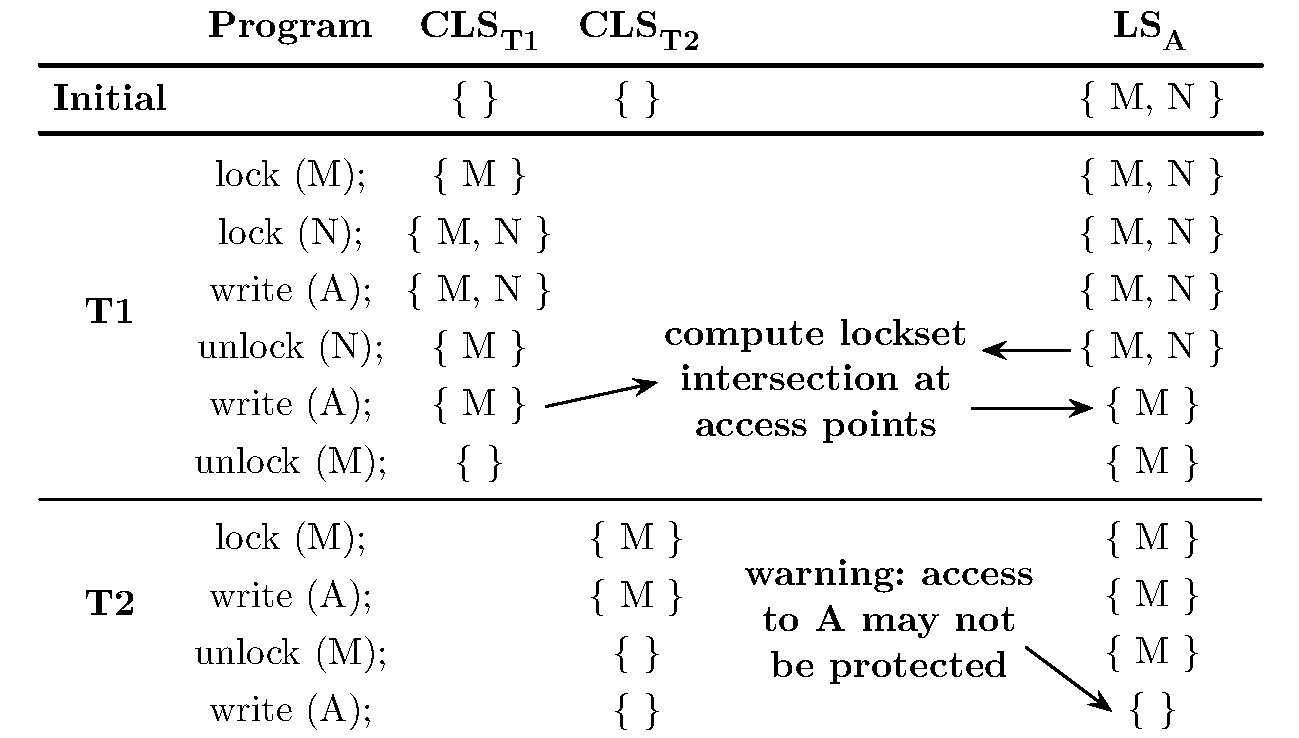
\includegraphics[width=1\linewidth]{img/lockset.pdf}
%\vspace{-5mm}
\caption{Applying lockset analysis on a concurrent program.}
\label{fig:locksets}
%\vspace{-3mm}
\end{figure}


\section{Static Pairwise Lockset Analysis}
\label{main_technique}

We propose \emph{static pair-wise lockset analysis}, a novel verification technique for proving data race freedom in device drivers. The key idea behind our approach is that we can verify absence of data races by (i) deriving a sound \emph{sequential} model that \emph{over-approximates} the originally concurrent driver, (ii) instrumenting it for lockset analysis and race checking, and (iii) asserting that all write/read accesses to the same shared resource are consistently protected by at least one common lock. The immediate benefit is that our approach not only avoids reasoning about thread interleavings, and thus has the potential to scale well, but also allows the reuse of existing successful sequential verification techniques.

The proof sketch behind our static lockset analysis is given in Section~\ref{proof}. The verification technique is described in more detail in Section~\ref{method}. The prototype implementation of our approach as the practical tool \textsc{Whoop} is presented in Section~\ref{implementation}.

\subsection{Static lockset analysis proof sketch}
\label{proof}

We now formalise our approach to verifying data race freedom in a device driver by statically analysing its locksets. Let $\{\mathit{ep}_{1}, \mathit{ep}_{2}, \dotsc, \mathit{ep}_{n}\}$ be all the entry points of a driver, and let $\{\ell_{1}, \ell_{2}, \dotsc, \ell_{k}\}$ be all the locks used by this driver. Although we assume that the number of locks is finite and with a known bound, we argue that this assumption is realistic: all device drivers that we have studied so far in the Linux kernel have only a small number of locks (typically one). Indeed, the Linux device driver book~\cite{corbet2005linux} advocates the use of as few locks as possible to avoid introducing unnecessary complexity and synchronisation bugs that arise from careless fine-grained locking. 

For each entry point $\mathit{ep}_{i}$, we compute its lockset $\mathit{LS}_{i}$ that associates each memory location $m$ to the set of locks that are always held when $m$ is accessed during the execution of $\mathit{ep}_{i}$. Furthermore, for each entry point $\mathit{ep}_{i}$, we compute $W_{i}\lbrack m\rbrack \rightarrow \{true, false\}$, which maps each $m$ to true if and only if $\mathit{ep}_{i}$ writes to $m$ during some execution.

\begin{theorem}
\label{theorem:locksets}
For each pair of entry points $\mathit{ep}_{i}, \mathit{ep}_{j}\in \{\mathit{ep}_{1}, \mathit{ep}_{2}, ..., \mathit{ep}_{n}\}$, where $i$ may be equal to $j$, and for each memory location $m$, if $(W_{i}\lbrack m\rbrack \vee W_{j}\lbrack m\rbrack) \implies (\mathit{LS}_{i}\lbrack m\rbrack \cap \mathit{LS}_{j}\lbrack m\rbrack \not= \varnothing)$, then the device driver with entry points $\{\mathit{ep}_{1}, \mathit{ep}_{2}, \dotsc, \mathit{ep}_{n}\}$ is free from data races.
\end{theorem}

A sketch of how the above theorem can be proved is as follows. Suppose there are in fact entry points $\mathit{ep}_{i}$ and $\mathit{ep}_{j}$ that can race on a memory location $m$. By our hypothesis, there exists at least one lock, say $\ell$, which belongs to both $\mathit{LS}_{i}$ and $\mathit{LS}_{j}$. By the definition of a lockset, this means that $\ell$ is held during the access to $m$ by both entry points $ep_1$ and $ep_2$. As a result, $m$ \emph{must} be unlocked and locked between the two accesses, which contradicts that the pair of accesses is racing.

\subsection{Verification method}
\label{method}

\begin{table*}
\small
\begin{center}
\begin{tabular}{lll}
\textbf{Statement}           & \textbf{Logger's Instrumentation}      & \textbf{Checker's Instrumentation} \\
\noalign{\smallskip}\toprule
\textbf{lock}(m);              & \textbf{add\_lock}(CL, m);                        & \textbf{add\_lock}(CL, m); \\
\noalign{\smallskip}\hline\noalign{\smallskip}
\textbf{unlock}(m);          & \textbf{remove\_lock}(CL, m);                  & \textbf{remove\_lock}(CL, m); \\
\noalign{\smallskip}\hline\noalign{\smallskip}
\multirow{2}{*}{x := *ptr;} & LS$\lbrack $ptr$\rbrack :=$ LS$\lbrack $ptr$\rbrack$ $\cap$ CL; & \textbf{assert}(W$\lbrack $ptr$\rbrack \implies$ CL $\cap$ LS$\lbrack $ptr$\rbrack \not= \varnothing$); \\
\noalign{\smallskip}
                                       & \textbf{havoc}(x);                                 & \textbf{havoc}(x); \\
\noalign{\smallskip}\hline\noalign{\smallskip}
\multirow{2}{*}{*ptr := x;} & LS$\lbrack $ptr$\rbrack :=$ LS$\lbrack $ptr$\rbrack$ $\cap$ CL; & \multirow{2}{*}{\textbf{assert}(CL $\cap$ LS$\lbrack $ptr$\rbrack \not= \varnothing$);} \\
\noalign{\smallskip}
                                       & W$\lbrack $ptr$\rbrack := true;$ &
\end{tabular}
\end{center}
\caption{Logger and Checker statements to be instrumented in each pair of entry points. The \texttt{havoc(x)} statement assigns a nondeterministic value to \texttt{x}.}
\label{tab:instrumentation}
\end{table*}

Our approach begins by performing \emph{two-thread reduction}, an abstraction that removes all but two arbitrary threads, each running an entry point of the originally concurrent driver, and then performs \emph{pair-wise sequentialisation}, which combines the two arbitrary threads in a single sequential pair. This is achieved by replacing the \texttt{return} statement of the first entry point with a \texttt{goto} statement that jumps execution to the first statement of the second entry point. This process repeats until all pairs of entry points have been sequentialised. To achieve soundness, each time an entry point performs a read access to a shared resource, we return a nondeterministic value. This over-approximates any effects from all the unmodeled threads on the device driver shared state.

Next, we split each pair into two distinct analysis regions: the \emph{logger}, which contains all the statements from the first entry point; and the \emph{checker}, which contains all the statements from the second entry point. The logger and the checker are then instrumented according to Table~\ref{tab:instrumentation}. The two regions directly contribute to the static lockset analysis and race checking as follows: the logger is responsible for recording all locksets $\mathit{LS}$ maintained by its entry point; while the checker asserts for potential conflicts between its own entry point and a given lockset $\mathit{LS}$ from the logger. This whole process is summarised below:

\begin{description}
  \item[Logger] Initially, for each memory location $m$ accessed by the logger's entry point, the logger's lockset $\mathit{LS}\lbrack m\rbrack$ contains all locks $\ell$ in the device driver, while the write access set $W\lbrack m\rbrack$ is set to false. Also, the logger's current lockset $\mathit{LS}_{CR}$, which is the set of all locks \emph{currently} held by the logger's entry point, is initially empty. Each time the logger performs a read or write access to $m$, it updates its lockset $\mathit{LS}\lbrack m\rbrack$, with the intersection of $\mathit{LS}\lbrack m\rbrack$ and $\mathit{LS}_{CR}$. This process is known as \emph{lockset refinement}~\cite{savage1997eraser} and results into a $\mathit{LS}\lbrack m\rbrack$ that contains only the locks $\ell$ that consistently protect $m$ during the execution of the logger's entry point.
  
  \item[Checker] Initially, for each memory location $m$ accessed by the checker's entry point, the checker's lockset $\mathit{LS}\lbrack m\rbrack$ and write access set $W\lbrack m\rbrack$ are equal to the corresponding sets supplied at the end of the logger. Also, the logger's current lockset $\mathit{LS}_{CR}$ is initially empty. Each time the checker performs a write access to $m$, it asserts that the intersection between $\mathit{LS}_{CR}$ and $\mathit{LS}\lbrack m\rbrack$ is non-empty. If the assertion fails, it implies that the entry point of the logger and the entry point of the checker potentially race on $m$. In this case a counterexample is generated and reported to the user. To check a read access, the checker performs the aforementioned assertion only if the write access set $W\lbrack m\rbrack$ is true, thus avoids to report a read-read data race, which is inherently benign.
\end{description}

\section{Implementation}
\label{implementation}

We have prototyped static pair-wise lock set analysis in \textsc{Whoop}, a practical tool for automatic verification of data race freedom in Linux drivers written in C~\cite{kernighan1988c}.

Initially, the device driver source code, together with a Linux environmental model\footnote{Stub header files required for compiling and subsequently analysing a device driver.}, is compiled to LLVM-IR using Clang/LLVM~\cite{lattner2004llvm}. Then, the LLVM-IR is compiled to the Boogie~\cite{barnett2006boogie} verification language using SMACK~\cite{rakamaric2008automatic}, an open source LLMV-IR to Boogie translator which can efficiently model heap manipulating programs. Next, the Boogie program is transformed into a sequentialised abstract program, using pair-wise sequentialisation and lock set instrumentation as discussed in Section~\ref{method}. Finally the abstract program is send to the Boogie verification engine, which generates verification conditions~\cite{barnett2005weakest} and discharges them to a theorem prover. Successful verification implies that the original driver is free of data races, while an error denotes a \emph{potential} data race.

\textsc{Whoop} is currently working on an unmodified network device driver (the RealTek r8169 which is part of the official Linux kernel distribution). Our immediate future work includes applying invariant generation to tame the effect of our coarse over-approximation. We also plan to introduce counterexample feasibility checking to evaluate if a reported bug is real or spurious. Towards this, we plan to feed a counterexample generated by \textsc{Whoop} into a precise bug finder, such as Corral~\cite{lal2012corral}, which will be guided only to execution paths that may manifest the bug, to either confirm it or discard it as a false positive.

\section{Evaluation}

\newcommand{\colspacing}{\hspace{1.8em}}
\begin{table}[t]
\small
\centering
\setlength{\tabcolsep}{0.3em}
\caption{Program statistics and race-checking results from applying \whoop and \corral on our benchmarks.}
\label{tab:stats}
\begin{tabular}{l rrr rr r}
\centering
& & & & \multicolumn{2}{c}{\textbf{\whoop}}
& \textbf{\corral}\\
\cmidrule(lr){5-6}
\cmidrule(lr){7-7}

& & & & \multicolumn{1}{r}{\textbf{\#Racy}}
& \multicolumn{1}{r}{\textbf{\#Racy}}
& \multicolumn{1}{r}{\textbf{\#Races}}\\

\textbf{Benchmarks}
& \textbf{LoC}
& \textbf{\#Pairs}
& \textbf{\#MRs}
& \multicolumn{1}{r}{\textbf{Pairs}}
& \multicolumn{1}{r}{\textbf{MRs}}
& \multicolumn{1}{r}{\textbf{Found}}\\[0.3em]

\toprule

generic\_nvram
& 283
& 14
& 39
& \multicolumn{1}{r}{7}
& \multicolumn{1}{r}{2}
& 4\\

pc8736x\_gpio
& 354
& 27
& 55
& \multicolumn{1}{r}{13}
& \multicolumn{1}{r}{6}
& 5\\

machzwd
& 457
& 10
& 49
& \multicolumn{1}{r}{6}
& \multicolumn{1}{r}{3}
& 1\\

ssu100
& 568
& 7
& 27
& \multicolumn{1}{r}{\xmark}
& \multicolumn{1}{r}{\xmark}
& \xmark\\

intel\_scu\_wd
& 632
& 10
& 45
& \multicolumn{1}{r}{5}
& \multicolumn{1}{r}{1}
& 2\\

ds1286
& 635
& 15
& 49
& \multicolumn{1}{r}{5}
& \multicolumn{1}{r}{3}
& \xmark\\

dtlk
& 750
& 21
& 53
& \multicolumn{1}{r}{10}
& \multicolumn{1}{r}{6}
& \xmark\\

fs3270
& 883
& 15
& 54
& \multicolumn{1}{r}{9}
& \multicolumn{1}{r}{1}
& \xmark\\

gdrom
& 890
& 94
& 41
& \multicolumn{1}{r}{21}
& \multicolumn{1}{r}{2}
& \xmark\\

swim
& 996
& 28
& 80
& \multicolumn{1}{r}{15}
& \multicolumn{1}{r}{7}
& 8\\

intel\_nfcsim
& 1272
& 10
& 24
& \multicolumn{1}{r}{10}
& \multicolumn{1}{r}{2}
& \xmark\\

ps3vram
& 1499
& 4
& 32
& \multicolumn{1}{r}{1}
& \multicolumn{1}{r}{1}
& \xmark\\

sonypi
& 1729
& 30
& 62
& \multicolumn{1}{r}{19}
& \multicolumn{1}{r}{4}
& 2\\

sx8
& 1751
& 2
& 47
& \multicolumn{1}{r}{2}
& \multicolumn{1}{r}{1}
& 1\\

8139too
& 2694
& 46
& 37
& \multicolumn{1}{r}{40}
& \multicolumn{1}{r}{4}
& \xmark\\

r8169
& 7205
& 192
& 50
& \multicolumn{1}{r}{88}
& \multicolumn{1}{r}{1}
& \xmark\\

\bottomrule
\end{tabular}
\end{table}

\begin{table*}[t]
\small
\centering
\setlength{\tabcolsep}{0.45em}
\caption{Comparison with different yield instrumentation granularities and context-switch bounds.}
\label{tab:results}
\begin{tabular}{l r rrrr rrrr rrrr}
\centering
& \textbf{\whoop}
& \multicolumn{3}{c}{\textbf{\corral}}
& \multicolumn{6}{c}{\textbf{\whoop + \corral}}\\
\cmidrule(lr){2-2}
\cmidrule(lr){3-5}
\cmidrule(lr){6-11}

& \multirow{2}{*}{\textbf{Time}}
& \multicolumn{3}{c}{\textbf{\yieldall\xspace --- Time (sec)}}
& \multicolumn{3}{c}{\textbf{\yieldcoarse\xspace --- Time (sec)}}
& \multicolumn{3}{c}{\textbf{\yieldmr\xspace --- Time (sec)}}\\
\cmidrule(lr){3-5}
\cmidrule(lr){6-8}
\cmidrule(lr){9-11}

\textbf{Benchmarks}
& \textbf{\textbf{(sec)}}
& \multicolumn{1}{r}{\textbf{csb = 2}}
& \multicolumn{1}{r}{\textbf{csb = 5}}
& \multicolumn{1}{r}{\textbf{csb = 9}}
& \multicolumn{1}{r}{\textbf{csb = 2}}
& \multicolumn{1}{r}{\textbf{csb = 5}}
& \multicolumn{1}{r}{\textbf{csb = 9}}
& \multicolumn{1}{r}{\textbf{csb = 2}}
& \multicolumn{1}{r}{\textbf{csb = 5}}
& \multicolumn{1}{r}{\textbf{csb = 9}}\\[0.3em]

\toprule

generic\_nvram
& \multicolumn{1}{r}{2.7}
& \multicolumn{1}{r}{27.9}
& \multicolumn{1}{r}{38.4}
& \multicolumn{1}{r}{146.2}
& \multicolumn{1}{r}{17.6}
& \multicolumn{1}{r}{22.2}
& \multicolumn{1}{r}{90.8}
& \multicolumn{1}{r}{14.2}
& \multicolumn{1}{r}{16.5}
& \multicolumn{1}{r}{42.0}\\

pc8736x\_gpio
& \multicolumn{1}{r}{5.3}
& \multicolumn{1}{r}{145.6}
& \multicolumn{1}{r}{302.0}
& \multicolumn{1}{r}{}
& \multicolumn{1}{r}{89.5}
& \multicolumn{1}{r}{229.5}
& \multicolumn{1}{r}{}
& \multicolumn{1}{r}{41.7}
& \multicolumn{1}{r}{56.9}
& \multicolumn{1}{r}{426.6}\\

machzwd
& \multicolumn{1}{r}{}
& \multicolumn{1}{r}{}
& \multicolumn{1}{r}{}
& \multicolumn{1}{r}{}
& \multicolumn{1}{r}{}
& \multicolumn{1}{r}{}
& \multicolumn{1}{r}{}
& \multicolumn{1}{r}{}
& \multicolumn{1}{r}{}
& \multicolumn{1}{r}{}\\

ssu100
& \multicolumn{1}{r}{}
& \multicolumn{1}{r}{}
& \multicolumn{1}{r}{}
& \multicolumn{1}{r}{}
& \multicolumn{1}{r}{}
& \multicolumn{1}{r}{}
& \multicolumn{1}{r}{}
& \multicolumn{1}{r}{}
& \multicolumn{1}{r}{}
& \multicolumn{1}{r}{}\\

intel\_scu\_wd
& \multicolumn{1}{r}{}
& \multicolumn{1}{r}{}
& \multicolumn{1}{r}{}
& \multicolumn{1}{r}{}
& \multicolumn{1}{r}{}
& \multicolumn{1}{r}{}
& \multicolumn{1}{r}{}
& \multicolumn{1}{r}{}
& \multicolumn{1}{r}{}
& \multicolumn{1}{r}{}\\

ds1286
& \multicolumn{1}{r}{}
& \multicolumn{1}{r}{}
& \multicolumn{1}{r}{}
& \multicolumn{1}{r}{}
& \multicolumn{1}{r}{}
& \multicolumn{1}{r}{}
& \multicolumn{1}{r}{}
& \multicolumn{1}{r}{}
& \multicolumn{1}{r}{}
& \multicolumn{1}{r}{}\\

dtlk
& \multicolumn{1}{r}{}
& \multicolumn{1}{r}{}
& \multicolumn{1}{r}{}
& \multicolumn{1}{r}{}
& \multicolumn{1}{r}{}
& \multicolumn{1}{r}{}
& \multicolumn{1}{r}{}
& \multicolumn{1}{r}{}
& \multicolumn{1}{r}{}
& \multicolumn{1}{r}{}\\

fs3270
& \multicolumn{1}{r}{}
& \multicolumn{1}{r}{}
& \multicolumn{1}{r}{}
& \multicolumn{1}{r}{}
& \multicolumn{1}{r}{}
& \multicolumn{1}{r}{}
& \multicolumn{1}{r}{}
& \multicolumn{1}{r}{}
& \multicolumn{1}{r}{}
& \multicolumn{1}{r}{}\\

gdrom
& \multicolumn{1}{r}{}
& \multicolumn{1}{r}{}
& \multicolumn{1}{r}{}
& \multicolumn{1}{r}{}
& \multicolumn{1}{r}{}
& \multicolumn{1}{r}{}
& \multicolumn{1}{r}{}
& \multicolumn{1}{r}{}
& \multicolumn{1}{r}{}
& \multicolumn{1}{r}{}\\

swim
& \multicolumn{1}{r}{}
& \multicolumn{1}{r}{}
& \multicolumn{1}{r}{}
& \multicolumn{1}{r}{}
& \multicolumn{1}{r}{}
& \multicolumn{1}{r}{}
& \multicolumn{1}{r}{}
& \multicolumn{1}{r}{}
& \multicolumn{1}{r}{}
& \multicolumn{1}{r}{}\\

intel\_nfcsim
& \multicolumn{1}{r}{}
& \multicolumn{1}{r}{}
& \multicolumn{1}{r}{}
& \multicolumn{1}{r}{}
& \multicolumn{1}{r}{}
& \multicolumn{1}{r}{}
& \multicolumn{1}{r}{}
& \multicolumn{1}{r}{}
& \multicolumn{1}{r}{}
& \multicolumn{1}{r}{}\\

ps3vram
& \multicolumn{1}{r}{}
& \multicolumn{1}{r}{}
& \multicolumn{1}{r}{}
& \multicolumn{1}{r}{}
& \multicolumn{1}{r}{}
& \multicolumn{1}{r}{}
& \multicolumn{1}{r}{}
& \multicolumn{1}{r}{}
& \multicolumn{1}{r}{}
& \multicolumn{1}{r}{}\\

sonypi
& \multicolumn{1}{r}{}
& \multicolumn{1}{r}{}
& \multicolumn{1}{r}{}
& \multicolumn{1}{r}{}
& \multicolumn{1}{r}{}
& \multicolumn{1}{r}{}
& \multicolumn{1}{r}{}
& \multicolumn{1}{r}{}
& \multicolumn{1}{r}{}
& \multicolumn{1}{r}{}\\

sx8
& \multicolumn{1}{r}{}
& \multicolumn{1}{r}{}
& \multicolumn{1}{r}{}
& \multicolumn{1}{r}{}
& \multicolumn{1}{r}{}
& \multicolumn{1}{r}{}
& \multicolumn{1}{r}{}
& \multicolumn{1}{r}{}
& \multicolumn{1}{r}{}
& \multicolumn{1}{r}{}\\

8139too
& \multicolumn{1}{r}{}
& \multicolumn{1}{r}{}
& \multicolumn{1}{r}{}
& \multicolumn{1}{r}{}
& \multicolumn{1}{r}{}
& \multicolumn{1}{r}{}
& \multicolumn{1}{r}{}
& \multicolumn{1}{r}{}
& \multicolumn{1}{r}{}
& \multicolumn{1}{r}{}\\

r8169
& \multicolumn{1}{r}{228.1}
& \multicolumn{1}{r}{T.O.}
& \multicolumn{1}{r}{T.O.}
& \multicolumn{1}{r}{T.O.}
& \multicolumn{1}{r}{28755.2}
& \multicolumn{1}{r}{T.O.}
& \multicolumn{1}{r}{T.O.}
& \multicolumn{1}{r}{26939.4}
& \multicolumn{1}{r}{T.O.}
& \multicolumn{1}{r}{T.O.}\\

\bottomrule
\end{tabular}
\end{table*}

\begin{figure}
\centering
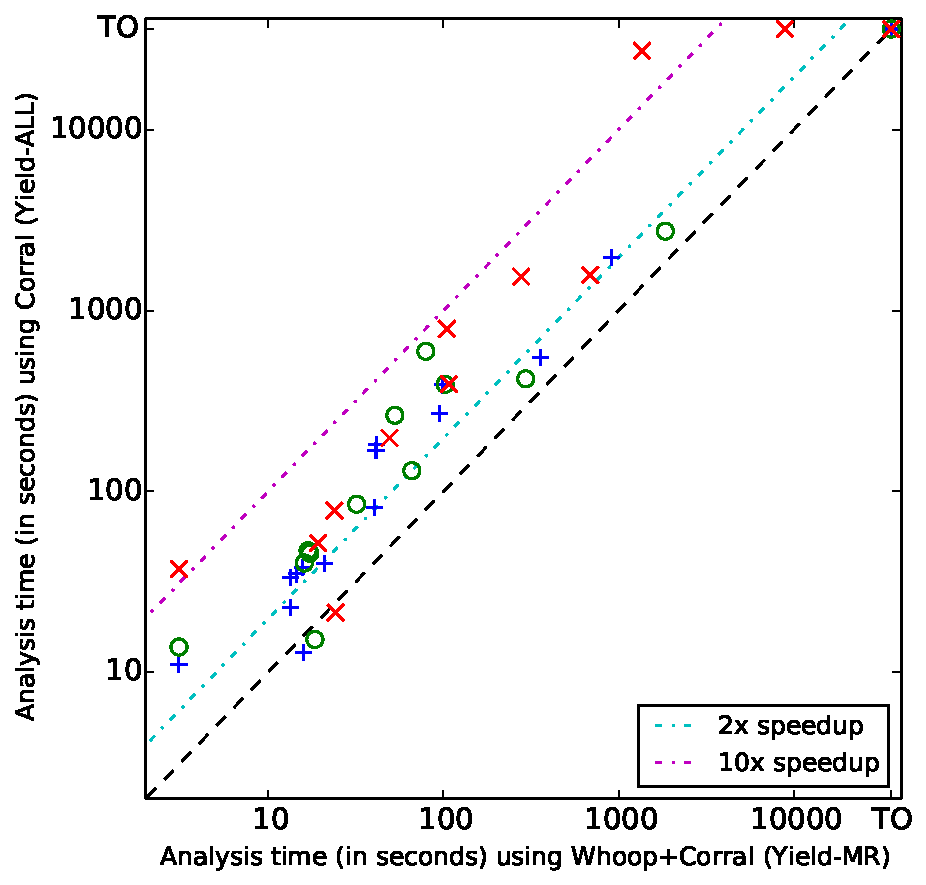
\includegraphics[width=.99\linewidth]{experiments/figures/yieldmr_vs_yieldall.pdf}
\caption{Scatter plot showing the runtime speedups that \corral achieves using \whoop with the \yieldmr instrumentation. The symbols $+$, $\circ$ and $\times$, represent a context-switch bound of 2, 5 and 9, respectively.}
\label{fig:plot}
\end{figure}

We performed experiments to validate the usefulness of the \whoop approach (Section~\ref{whoop}) and its combination with \corral (Section~\ref{corral}). We first present race-checking results from running \whoop and \corral on \sizeOfBenchmarks drivers taken from the 4.0 Linux kernel distribution.\footnote{\url{https://www.kernel.org}} We then evaluate the runtime performance and scalability of \corral and \whoop + \corral with different yield instrumentation granularities and context-switch bounds.
Our results demonstrate that \whoop can efficiently accelerate race-checking with \corral.

\noindent
\textbf{Experimental Setup}\xspace\xspace We performed all experiments on a 3.40GHz Intel Core i7-2600 CPU with 16GB RAM running Ubuntu Linux 12.04.5 LTS, LLVM 3.5, SMACK 1.5, Z3 4.3.2, Boogie rev. 4192 and \corral rev. 534.  \ADComment{Perhaps also state that Boogie runs inside Mono, and give the Mono version?}

\noindent
\textbf{Benchmarks}\xspace\xspace We evaluate our methodology against \sizeOfBenchmarks drivers taken from the 4.0 Linux kernel. We chose non-trivial drivers from several domains: block; char; ethernet; near field communication (nfc); universal serial bus (usb); and watchdog. We had to manually model the environment for these drivers, a process that required approximately two months of work.  \ADComment{Question from me: are block and char domains, in the same way that ethernet is a domain?}

\ADComment{At this point, is it absolutely clear what we do with \corral?  I.e., that we consider each entry point pair separately, and do not employ any abstraction to model additional threads?}

\noindent
\textbf{Race-Checking}\xspace\xspace Table~\ref{tab:stats} presents statistics for all our benchmarks: lines of code (LoC); number of entry point pairs (\#Pairs); number of SMACK memory regions (\#MRs); number of potentially racy pairs identified by \whoop (\#Racy Pairs); number of potentially racy memory regions reported by \whoop (\#Racy MRs); and number of races discovered by \corral using a context-switch bound of 2 (\#Races Found). We did not discover new races with larger context-switch bounds. This might mean that these drivers only have races that manifest with at least one or two context-switches, or that \corral hit its bounds before discovering a deeper race.

We can see that \whoop reports more races than \corral. This is expected, since \whoop employs an over-approximating shared state abstraction to conservatively model the effects of additional threads when analysing an entry point pair, and because lockset analysis is inherently imprecise; both factors can lead to false alarm race reports.  On the other hand, \corral is precise, but can miss races because only a limited number of context switches are considered.  Another issue with \corral is loop coverage due to unsound loop unrolling. To tackle this, we enable the built-in loop over-approximation described in~\cite{lal2014powering}. This can potentially lead \corral to report false positives, but we have not seen this in practice.  \ADComment{Would this be a good point to reiterate the fact that when we apply \corral to an entry point pair, we are just checking the specific pair of threads, and are not accounting for actions by other threads?}

Most of the races that \whoop and \corral discovered can be classified in two cases. The first case is accessing a global counter (or flag) from concurrent entry points, without a lock. This might be for performance, and indeed a lot of the races we found might be benign. Even benign races, though, lead to undefined behavior according to the C standard, and it is well known that undefined behaviors can lead to unexpected results when combined with aggressive compiler optimizations. The second case is an entry point accessing a field of an object (either global or passed as a parameter) without a lock. This can lead to a race if another entry point simultaneously accesses the same field of the same object.

As an example of the second case, we found the following race in the generic\_nvram char driver (see Figure~\ref{fig:data_race_example} for the source code): during the \texttt{llseek} entry point, the driver is accessing the file offset \texttt{file->f\_pos} without first acquiring a lock (\texttt{file} is passed as a parameter to \texttt{llseek}). This can lead to a race if the driver invokes \texttt{llseek} from another thread passing the same \texttt{file} object as a parameter. When we investigated another char driver that uses the same APIs, we saw that it was protecting the offset access in its \texttt{llseek} entry point with a mutex. This made us suspicious that the race we found in generic\_nvram could be real. We filed a bug report, but did not manage to get a response yet.

\noindent
\textbf{Granularity of Context-Switches}\xspace\xspace Table~\ref{tab:results} presents runtime results from using \whoop, \corral and \whoop + \corral to analyze our benchmarks. All reported times, in seconds, are averages over three runs. \ADComment{Can we say something about variance?  Perhaps ask Nathan what best to say?} \corral was given a time budget of 10 hours (T.O. denotes a tool timeout), and we considered context-switch bounds (csb) of 2, 5 and 9. By default, \corral instruments context-switches (i.e. \texttt{yield} statements) in \ADComment{instead of ``in'' can we say either ``before'' or ``after'' (not sure which is accurate)} all visible operations (denoted \yieldall). \whoop + \corral, instead, uses two different context-switch instrumentation granularities, \yieldcoarse and \yieldmr (see Section~\ref{whoop:bugfinding}), and also uses all the optimisations discussed in Section~\ref{whoop:optimizations}.

A higher context-switch bound results into deeper interleavings being explored and thus a larger sequentialized program. Intuitively, this means that we see even greater speedups using information from \whoop, when exploring deeper interleavings.

We can notice that \whoop is significantly faster than \corral. This is expected as \whoop achieves scalability using over-approximation and summarization techniques. This allows \whoop to perform especially well in complex drivers such as the r8169 ethernet driver: although \corral ... and timeouts with a csb of 9, \whoop manages to analyze the driver in 228.1 seconds. We believe that the reason behind this is that r8169 has many loops and uses deeply-nested recursion in some entry points, which \corral might not be able to handle efficiently.

%When running \corral on its own, it can potentially report a spurious race (that \whoop does not report), because \corral is not enhanced with domain-specific information that \whoop uses to discard spurious races. Using \whoop + \corral, though, will inherently discard spurious data races (assuming a precise environmental model).

%When \corral on its own tries to analyze the machzwd watchdog driver it explodes, because in some entry point pairs it attempts to analyze a large number of memory regions. For example for the entry point pair write vs init, it instruments interleavings at 26 different memory regions in a single invocation of \corral, which required approximately 1000 seconds to analyze. The same entry point pair is found race-free by \whoop. Using this information in \corral with the \yieldmr instrumentation, the pair takes less than a second to analyze. The \yieldcoarse instrumentation does not perform as well, because it works in the binary granularity of racy or non-racy entry points.


\section{Related Work}

Statically analyzing concurrent programs to detect races is a promising alternative to dynamic analyzers, which commonly face code coverage issues as they rely on a (controlled) scheduler for exploring execution paths~\cite{musuvathi2008finding}. Warlock~\cite{sterling1993warlock} and LockLint~\cite{oracle2010locklint} are notable examples of static race analyzers. However, both tools have limited applicability, as they heavily rely on user annotations. \textsc{Whoop}, on the other hand, does not require any source code modifications, and thus can be applied with minimal effort.

Most related to our work are the static lockset analyzers RELAY~\cite{voung2007relay} and Locksmith~\cite{pratikakis2006locksmith}. Both tools, though, have significant limitations. The authors of RELAY found 5022 warnings when analyzing the Linux kernel, with only 25 of them being true data races. To limit these false positives, RELAY employs post-analysis unsound filters, but these can also filter out true races. Although Locksmith successfully detected data races in several small Pthreads applications and 7 medium-sized Linux device drivers, it also reported a significant number of false positives. The authors also reported that Locksmith was unable to run on several large programs, showcasing its limited scalability. In contrast, \whoop is based on novel over-approximation techniques and uses modern SMT solvers to accelerate state-of-the-art concurrency bug-finders, such as \corral, for precise \emph{and} scalable analysis.

\section{Conclusions}

In this paper, we presented \whoop, a novel infrastructure for (i) analyzing the concurrent behavior of Linux drivers and (ii) accelerating a plugged-in bug-finder using information from our static data race analysis. In the heart of our approach, we combine static lock set analysis with sound sequentialization and automated theorem proving. Our lock set analysis enforces the locking discipline that two threads accessing the same shared resource must hold at least one common lock, and reports a potential data race if this discipline is violated.

Compared to traditional data race detection tools that typically attempt to explore as many thread interleavings as feasible, and thus face scalability issues in the presence of realistic concurrent programs, \textsc{Whoop} not only entirely avoids reasoning about thread interleavings, but also allows the reuse of existing successful sequential verification techniques. The main limitation of our approach is that it can potentially report many false positives, as we over-approximate the device driver shared state. To tackle this problem, we use the race-related information that \whoop generates to speed up \corral, a state-of-the-art precise bug-finder for concurrent programs.

% An example of a floating figure using the graphicx package.
% Note that \label must occur AFTER (or within) \caption.
% For figures, \caption should occur after the \includegraphics.
% Note that IEEEtran v1.7 and later has special internal code that
% is designed to preserve the operation of \label within \caption
% even when the captionsoff option is in effect. However, because
% of issues like this, it may be the safest practice to put all your
% \label just after \caption rather than within \caption{}.
%
% Reminder: the "draftcls" or "draftclsnofoot", not "draft", class
% option should be used if it is desired that the figures are to be
% displayed while in draft mode.
%
%\begin{figure}[!t]
%\centering
%\includegraphics[width=2.5in]{myfigure}
% where an .eps filename suffix will be assumed under latex, 
% and a .pdf suffix will be assumed for pdflatex; or what has been declared
% via \DeclareGraphicsExtensions.
%\caption{Simulation Results}
%\label{fig_sim}
%\end{figure}

% Note that IEEE typically puts floats only at the top, even when this
% results in a large percentage of a column being occupied by floats.


% An example of a double column floating figure using two subfigures.
% (The subfig.sty package must be loaded for this to work.)
% The subfigure \label commands are set within each subfloat command, the
% \label for the overall figure must come after \caption.
% \hfil must be used as a separator to get equal spacing.
% The subfigure.sty package works much the same way, except \subfigure is
% used instead of \subfloat.
%
%\begin{figure*}[!t]
%\centerline{\subfloat[Case I]\includegraphics[width=2.5in]{subfigcase1}%
%\label{fig_first_case}}
%\hfil
%\subfloat[Case II]{\includegraphics[width=2.5in]{subfigcase2}%
%\label{fig_second_case}}}
%\caption{Simulation results}
%\label{fig_sim}
%\end{figure*}
%
% Note that often IEEE papers with subfigures do not employ subfigure
% captions (using the optional argument to \subfloat), but instead will
% reference/describe all of them (a), (b), etc., within the main caption.


% An example of a floating table. Note that, for IEEE style tables, the 
% \caption command should come BEFORE the table. Table text will default to
% \footnotesize as IEEE normally uses this smaller font for tables.
% The \label must come after \caption as always.
%
%\begin{table}[!t]
%% increase table row spacing, adjust to taste
%\renewcommand{\arraystretch}{1.3}
% if using array.sty, it might be a good idea to tweak the value of
% \extrarowheight as needed to properly center the text within the cells
%\caption{An Example of a Table}
%\label{table_example}
%\centering
%% Some packages, such as MDW tools, offer better commands for making tables
%% than the plain LaTeX2e tabular which is used here.
%\begin{tabular}{|c||c|}
%\hline
%One & Two\\
%\hline
%Three & Four\\
%\hline
%\end{tabular}
%\end{table}


% Note that IEEE does not put floats in the very first column - or typically
% anywhere on the first page for that matter. Also, in-text middle ("here")
% positioning is not used. Most IEEE journals/conferences use top floats
% exclusively. Note that, LaTeX2e, unlike IEEE journals/conferences, places
% footnotes above bottom floats. This can be corrected via the \fnbelowfloat
% command of the stfloats package.


% use section* for acknowledgement
\section*{Acknowledgments}
We would like to thank the Multicore Programming Group of Imperial College London for all the useful discussions and feedback. This work is part of the research project ``Automatic Synthesis of High-Assurance Device Drivers'' and is generously funded by a gift from Intel Corporation.


% trigger a \newpage just before the given reference
% number - used to balance the columns on the last page
% adjust value as needed - may need to be readjusted if
% the document is modified later
%\IEEEtriggeratref{8}
% The "triggered" command can be changed if desired:
%\IEEEtriggercmd{\enlargethispage{-5in}}

% references section

% can use a bibliography generated by BibTeX as a .bbl file
% BibTeX documentation can be easily obtained at:
% http://www.ctan.org/tex-archive/biblio/bibtex/contrib/doc/
% The IEEEtran BibTeX style support page is at:
% http://www.michaelshell.org/tex/ieeetran/bibtex/
\bibliographystyle{IEEEtran}
% argument is your BibTeX string definitions and bibliography database(s)
\bibliography{references}
%
% <OR> manually copy in the resultant .bbl file
% set second argument of \begin to the number of references
% (used to reserve space for the reference number labels box)
%\begin{thebibliography}{1}

%\bibitem{IEEEhowto:kopka}
%H.~Kopka and P.~W. Daly, \emph{A Guide to \LaTeX}, 3rd~ed.\hskip 1em plus
 % 0.5em minus 0.4em\relax Harlow, England: Addison-Wesley, 1999.

%\end{thebibliography}




% that's all folks
\end{document}


